\documentclass{cmn}

\begin{document}
  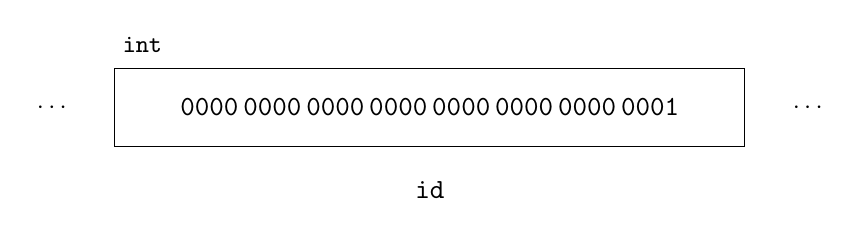
\begin{tikzpicture}
    \draw (-2*16mm,0) -- ++(5*16mm,0) -- ++(0,10mm) -- ++(-5*16mm,0) -- cycle;

    \node at (-2*16mm-8mm,5mm) {\small$\cdots$};
    \node at (3*16mm+8mm,5mm) {\small$\cdots$};

    \node at (8mm,5mm) {\texttt{0000{\,}0000{\,}0000{\,}0000{\,}0000{\,}0000{\,}0000{\,}0001}};
    \node at (5mm-1.5mm-2*16mm,10mm+3mm) {\small\texttt{int}};
    \node at (8mm,-5.5mm) {\texttt{id}};
  \end{tikzpicture}
\end{document}
